\documentclass[15pt,a5paper,reqno]{article}
\usepackage{hyperref}
\usepackage[warn]{mathtext}
\usepackage[utf8x]{inputenc}
\usepackage{amssymb, amsmath, multicol}
\usepackage[russian]{babel}
\usepackage{graphicx}
\usepackage[shortcuts,cyremdash]{extdash}
\usepackage{wrapfig}
\usepackage{floatflt}
\usepackage{lipsum}
\usepackage{verbatim}
\usepackage{concmath}
\usepackage{euler}
\usepackage{xcolor}
\usepackage{etoolbox}
\usepackage{fancyhdr}
\usepackage{subfiles}
\usepackage{enumitem}
\usepackage{amsthm}
\usepackage{indentfirst}
\usepackage{import}

\DeclareMathOperator{\sign}{sign}

\RequirePackage[ left     = 1.5cm,
  right    = 1.5cm,
  top      = 2.0cm,
  bottom   = 1.25cm,
  includefoot,
  footskip = 1.25cm ]{geometry}
\setlength    {\parskip}        { .5em plus .15em minus .08em }
%\setlength    {\parindent}      { .0em }
\renewcommand {\baselinestretch}{ 1.07 }

\fancyhf{}

\renewcommand{\footrulewidth}{ .0em }
\fancyfoot[C]{\texttt{\textemdash~\thepage~\textemdash}}
\fancyhead[R]{\hfilШурыгин Антон}

\makeatletter
\patchcmd\l@section{%
  \nobreak\hfil\nobreak
}{%
  \nobreak
  \leaders\hbox{%
    $\m@th \mkern \@dotsep mu\hbox{.}\mkern \@dotsep mu$%
  }%
  \hfill
  \nobreak
}{}{\errmessage{\noexpand\l@section could not be patched}}
\makeatother
\parindent = 1cm % отступ при красной строке⏎
\pagestyle{fancy}    
\renewcommand\qedsymbol{$\blacksquare$}

\newcommand{\when}[2]{
  \left. #1 \right|_{#2} \hspace
}
\renewcommand{\kappa}{\varkappa}
\RequirePackage{caption2}
\renewcommand\captionlabeldelim{}
\newcommand*{\hm}[1]{#1\nobreak\discretionary{}

\DeclareSymbolFont{T2Aletters}{T2A}{cmr}{m}{it}

{\hbox{$\mathsurround=0pt #1$}}{}}
% Цвета для гиперссылок
\definecolor{linkcolor}{HTML}{000000} % цвет ссылок
\definecolor{urlcolor}{HTML}{799B03} % цвет гиперссылок
 
\hypersetup{pdfstartview=FitH,  linkcolor=linkcolor,urlcolor=urlcolor, colorlinks=true}


%\setcounter{secnum[utf8x]depth}{0}

\begin{document}

% НАЧАЛО ТИТУЛЬНОГО ЛИСТА
\begin{center}
  {\small ФЕДЕРАЛЬНОЕ ГОСУДАРСТВЕННОЕ АВТОНОМНОЕ ОБРАЗОВАТЕЛЬНОЕ\\ УЧРЕЖДЕНИЕ ВЫСШЕГО ОБРАЗОВАНИЯ\\ МОСКОВСКИЙ ФИЗИКО-ТЕХНИЧЕСКИЙ ИНСТИТУТ\\ (НАЦИОНАЛЬНЫЙ ИССЛЕДОВАТЕЛЬСКИЙ УНИВЕРСИТЕТ)\\ ФИЗТЕХ-ШКОЛА РАДИОТЕХНИКИ И КИБЕРНЕТИКИ}\\
  \hfill \break
  \hfill \break
  \hfill \break
  \Huge{Геометрическая оптика.}\\
\end{center}

\hfill \break
\hfill \break
\hfill \break
\hfill \break
\hfill \break
\hfill \break

\begin{flushright}
  \normalsize{Работу выполнили:}\\
  \normalsize{\textbf{Шурыгин Антон Алексеевич, группа Б01-909}}\\
\end{flushright}

\begin{center}
  \normalsize{\textbf{Долгопрудный, 2021}}
\end{center}


\thispagestyle{empty} % выключаем отображение номера для этой страницы

% КОНЕЦ ТИТУЛЬНОГО ЛИСТА

\newpage
\thispagestyle{plain}
\tableofcontents
\thispagestyle{plain}
\newpage



\textbf{Цель работы:}
Определить фокусные расстояния собирающих и рассеивающих линз, смоделировать ход лучей в трубе Галилея, трубе Кеплера и микроскопе, определить их увеличение

\textbf{Оборудование}: оптическая скамья, набор линз, экран, осветитель со шкалой, 
зрительная труба, диафрагма, линейка.

\section{Введение и краткая теория}

В работе предлагается измерить фокусные расстояния линз, смоделировать трубу Кеплера, трубу Галилея
микроскоп и определить их увеличения.
\newline

\textbf{Сложенин центрированных оптических систем}
Пусть две центрированные системы имеют общую главную оптическую ось. Если известны параметры каждой системы, а также их взаимное расположение, то аналитическим расчётом или геометрическим
построением можно определить положение всех кардинальных точек
сложной оптической системы, состоящей из этих двух систем.

Рассматриваемая система схематически изображена на рис. 1.3.
Кардинальные точки первой и второй систем отмечены соответствующими нижними индексами. Штрихами выделены кардинальные точки
пространства изображений первой системы и аналогичные точки пространства предметов второй системы. 
Величина $\Delta = F2 - F′1$ представляет расстояние от заднего фокуса первой системы до переднего фокуса
второй системы и называется оптическим интервалом двух систем. 
В соответствии с принятым правилом знаков $\Delta > 0$, если падающий светидёт от фокуса $F′1$ к фокусу $F2$, как отмечено стрелкой на рис. 1.3, в
противоположном случае $\Delta < 0$. Заданием оптического интервала полностью определяется взаимное расположение складываемых систем.

\begin{figure}[h!]
    \centering
    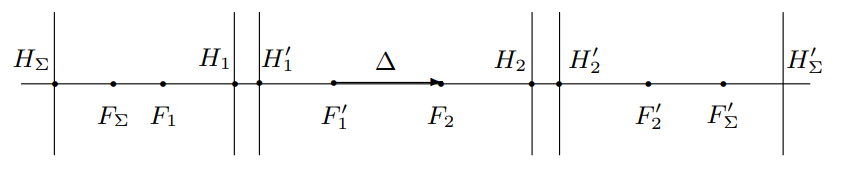
\includegraphics[width=0.8\linewidth]{pics/system_of_lens.png}
    \caption{Сложение центрированных систем}
    \label{}
\end{figure}


Конечные уравнения для фокусного расстояния и координат фокальных и главных точек сложной системы:


\begin{equation}\label{1}
    f_{\sum} = - \frac{f_1 f_2}{\Delta}
\end{equation}


\begin{equation}\label{2}
    f'_{\sum } = - \frac{f'_1 f'_2}{\Delta}
\end{equation}

\begin{equation}\label{3}
    \Phi = \frac{n}{f_{\sum}} = -\frac{n\Delta}{f_1 f_2}
\end{equation}



\textbf{Примеры центрированных оптических систем}
Оптическая система может не иметь фокальных плоскостей. Такая система называется афокальной или телескопической.
Она является предельным случаем обычной системы, у которой фокальные плоскости сдвинуты в беконечность.
Как видно из формул для сложных систем, телескопической становится система из двух обычных систем, если их оптический интервал $\Delta \rightarrow 0$

Выполнив этот предельный переход в уравнениях, получим формулы для преобразования координат и коэффициенты увеличений телескопической системы:

\[ \frac{x'}{x} = \frac{\delta x'}{\delta x} = \frac{f_2 f'_2}{f_1 f'_1} \]
\[ \frac{y'}{y} = \frac{n \alpha}{n' \alpha'} = \frac{f_2}{f'_1} \]
  

Из выражений выше следует, что в телескопической системе:
\begin{enumerate}
    \item всякий параллельный пучок света после прохождения через систему остаётся параллельным
    \item продольное, поперечное и угловое увеличения постоянны, то есть не зависят от положения предмета.
\end{enumerate}

Оптическая сила телескопической системы, как видно из формулы \ref{3}, равна нулю.


\section{Определение фокусных расстояний линз с помощью зрительной трубы}
\subsection{Определение фокусного расстояния собирающих линз}


Настроим зрительную трубу на бесконечность
Поставим положительную линзу на расстоянии от предмета примерно равном фокусному. На небольшом расстоянии от линзы закрепим трубу, настроенную на бесконечность,
и отцентрируем её по высоте. Диафрагма диаметром $d = 1$ см, надетая на ближнюю к осветителю линзу, уменьшит сферические аберрации и повысит чёткость изображения.

Передвигая линзу вдоль скамьи, получим в окуляре зрительной трубы изображение предмета — миллиметровой сетки. При этом расстояние между предметом и серединой тонкой линзы (между проточками на оправах) равно фокусному.

    \begin{table}[h!]
        \centering
            \begin{tabular}{| c | c | c | c |}

                \hline
                    $n$ & $F_1, cm$ & $F_2, cm$ &  тип линзы\\
                \hline
                    1 & 8 & 8.2 & соб. \\
                \hline
                    2 & 10 & 10 & соб.\\
                \hline
                    3 & 18,8 & 19,3  & соб. \\
                \hline
                    4 & 32,5 & 32,5 & соб. \\
                \hline
                    5 & -9 & -9 &  рас.\\
                \hline
                \end{tabular}
        \caption{Результаты измерения фокусных расстояний линз}
        \label{nu1}
    \end{table}
    

\subsection{Определение фокусного расстояния рассеивающей линзф}

Для определения фокусного расстояния тонкой отрицательной линзы сначала получим на экране увеличенное изображение сетки при помощи одной короткофокусной положительной линзы. Измерим расстояние между линзой и экраном $a_0 = 33.7$ см.
Разместим сразу за экраном трубу, настроенную на бесконечность, и закрпим её. Уберём экран и поставьте на его место исследуемую рассеивающую линзу (рис. 8). Перемещая рассеивающую линзу, найдите в окуляре зрительной трубы резкое изображение сетки. \par
Измерив расстояние между линзами $l = 24.7$ см, рассчитаем фокусное расстояние рассеивающей линзы $f = a_0 - l$.
Результаты измерения фокусного расстояния рассеивающих линз:

\begin{center}
    $f_{рас} = 33,7 - 24,7 \approx 9$ см
\end{center}


За погрешность измерений берем предел в 0.5 см, что логично из таблицы (1). Кроме того наложим ограничение в $0.05F$ для получения четкого изображения.

\begin{figure}[h!]
    \begin{center}
        \begin{minipage}[h!]{0.60\linewidth}
            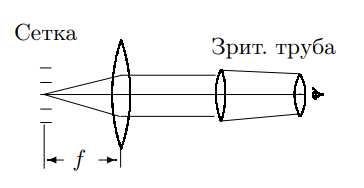
\includegraphics[width=1\linewidth]{pics/plus_lens.png}
            \caption{Определение фокусного расстояния собирающей линзы} %% подпись к рисунку
        \label{} 
        \end{minipage}

        \hfill 

        \begin{minipage}[h!]{0.60\linewidth}
            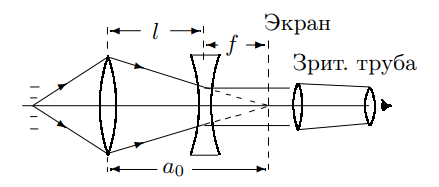
\includegraphics[width=1\linewidth]{pics/minus_lens.png}
            \caption{Определение фокусного расстояния рассеивающей линзы}
        \label{}
    \end{minipage}
    \end{center}
\end{figure}

\section{Моделирование трубы Кеплера}

Рассмотрим ход лучей в трубе Кеплера и найдём увеличение данной оптической системы:
    
\begin{figure}[h!]
    \centering
        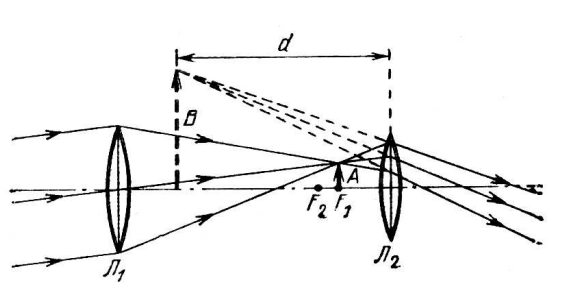
\includegraphics[width=10cm]{pics/kepler.png}
    \caption{Ход лучей в трубе Кеплера}
    \label{}
\end{figure}

Пусть пучок света, попадающий в объектив, составляет с оптической осью угол $\varphi_1$, а пучок, выходящий из окуляра, — угол $\varphi_2$. Увеличение $\gamma$ зрительной трубы по определению равно

\begin{equation}
    N = \frac{\tan \varphi_2}{\tan \varphi_1},
\end{equation}

но также из рис. 3 следует, что :

\begin{equation}
    N_{\tau} = -\frac{f_1}{f_2} = -\frac{D_1}{D_2},
\end{equation}

где $D_1$ - ширина пучка, прошедшего через объектив, а $D_2$ - ширина пучка, вышедшего из окуляра

Построим оптическую систему из каллиматора и непосредственно трубы Кеплера. 

\begin{figure}[h!]
        \centering
            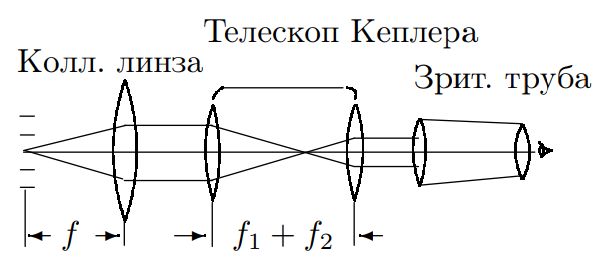
\includegraphics[width=10cm]{pics/kepler_2.png}
            \caption{Схема трубы Кеплера}
        \label{}
\end{figure}

Параметры действующих линз:

\begin{center}
    $f_{1} = 32.5$ см \hspace{1cm} $f_2 = 8$ см
\end{center}

Найдём увеличение трубы Кеплера непосредственно: пусть $h_1$ - размер ячейки миллиметровой сетки без телескопа, $h_2$ - с телескопом

\begin{center}
	$h_1 = 9$ мал. дел., \hspace{1cm} $h_2 = 34$ мал. дел. \par

	$N_{\tau} = -\frac{h_2}{h_1} \approx 3,7 \pm 0,53$
\end{center}

При этом по формуле (2) также

\begin{center}
    $N_{\tau} = -\frac{f_{1}}{f_2} \approx 4,06 \pm 0,51$
\end{center}

Кроме того существует еще один способ найти увеличение: частное $D_1 $ - диаметр объектива и $D_2$ - диаметр его изображения.

\begin{center}
	$N_{\tau} = -\frac{D_2}{D_1} = -\frac{3,4}{0,8} \approx -4,25 \pm 0,62$
\end{center}



\section{Моделирование трубы Галилея}
    \begin{figure}[h!]
    \centering
    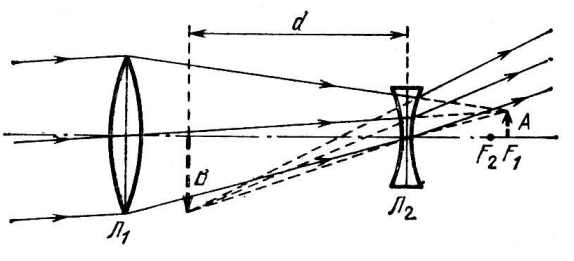
\includegraphics[width=9cm]{pics/gal.png}
    \caption{Ход лучей в трубе Галилея}
    \label{}
\end{figure}

Труба Галилея получается из трубы Кеплера заменой собирающей линзы окуляра рассеивающей. Формулы для увеличения, соответственно, остаются теми же:
\begin{equation}
    N_{\tau} = -\frac{f_1}{f_2} = -\frac{D_1}{D_2} =  -\frac{h_2}{h_1}
\end{equation}


Заменим собирающую линзу с фокусным расстоянием $f_2 = 8$ см рассеивающей с фокусным расстоянием $f_2 = 9$ см. Проведём те же операции, что и для трубы Кеплера:

\begin{center}
$h_1 = 9$ малых дел., \hspace{1cm} $h_2 = 30$ малых дел. \par
$N_{\tau} = -\frac{h_2}{h_1} \approx -3,33 \pm 0,46$
\end{center}

При этом выполняется так же:

\begin{center}
    $N_{\tau} = -\frac{f_1}{f_2} \approx -3,61 \pm 0,43$
\end{center}

Полученные значения хорошо совпадают.


\section{Моделирование микроскопа}

Для создания модели микроскопа с увеличением $N_M = -5$ (минус, т.к. изображение перевернуто) отберём самые короткофокусные линзы из набора. 
Рассчитаем необходимый интервал $\Delta$ и длину тубуса  $l_12$ по формулам:

\[ N_m = -\frac{\Delta}{f_1} \cdot \frac{L}{f_2} \: \rightarrow \: \Delta = -\frac{N_m f_1 f_2}{L}  \]


Где $L = 25$ см - расстояние наилучшего зрения нормального. 

\begin{figure}[h!]
    \centering
    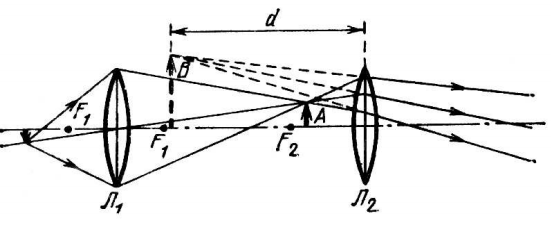
\includegraphics[width=9cm]{pics/micro.png}
    \caption{Ход лучей в микроскопе}
    \label{}
\end{figure}


Получаем, что $\Delta = 16$ см. Затем $l_12 = \Delta + f_1 + f_2$ = 34 см.
Таким образом:

\[   N_m = -\frac{h_2 L}{h_1 f} = -\frac{31 \cdot 25}{9 \cdot 18,8} \approx -4,58  \pm 1,02  \]


   
\section{Вывод}
В ходе работы были определены фокусные расстояния собирающих и рассеивающих линз с помощью зрительной трубы. 
\newline
Из этих линз далее сконструированы следующие оптические приборы: труба Кеплера, труба Галилея, микроскоп. 
\newline
Были определены их увеличения и проведено сравнение с её действительным значением. В пределах погрешности теоретическое значение хорошо совпадает с практическим.

\end{document}

